\documentclass{beamer}

% Should be documentclass beamer

\mode<presentation>
{
%  \usetheme[hideothersubsections]{PaloAlto}
  \usetheme{metropolis}
  \setbeamercovered{transparent}
}

\usepackage{amsfonts}
\usepackage{amsmath}
\usepackage{amssymb}
\usepackage{color}
\usepackage{tikz}
\usepackage{pgfplots}
\usepackage{listings}
\usepackage{courier}
%\usepackage[utf8]{inputenc}
%\usepackage[russian]{babel}

\lstset{
  numbers=left,
  basicstyle=\ttfamily\footnotesize,
  numberstyle=\tiny\color{gray},
  stepnumber=1,
  numbersep=10pt,
}

\newcommand{\iu}{\ensuremath{\mathrm{i}}}
\newcommand{\bbR}{\mathbb{R}}
\newcommand{\bbC}{\mathbb{C}}
\newcommand{\calV}{\mathcal{V}}
\newcommand{\calW}{\mathcal{W}}
\newcommand{\macheps}{\epsilon_{\mathrm{mach}}}
\newcommand{\matlab}{\textsc{Matlab}}

\newcommand{\ddiag}{\operatorname{diag}}
\newcommand{\fl}{\operatorname{fl}}
\newcommand{\nnz}{\operatorname{nnz}}
\newcommand{\tr}{\operatorname{tr}}
\renewcommand{\vec}{\operatorname{vec}}

\newcommand{\vertiii}[1]{{\left\vert\kern-0.25ex\left\vert\kern-0.25ex\left\vert #1
    \right\vert\kern-0.25ex\right\vert\kern-0.25ex\right\vert}}
\newcommand{\ip}[2]{\langle #1, #2 \rangle}
\newcommand{\ipx}[2]{\left\langle #1, #2 \right\rangle}
\newcommand{\order}[1]{O( #1 )}

\newcommand{\kron}{\otimes}


\newcommand{\hdr}[2]{
  \title[CS 5220, Fall 2017]{CS 5220: #2}
  \author{David Bindel}
  \date{#1}
}


\hdr{2017-11-16}{Impact of Floating Point}

\begin{document}

% Add discussion of reproducible BLAS, half precision arithmetic

\begin{frame}
  \titlepage
\end{frame}

\begin{frame}
  \frametitle{Why this lecture?}

  Isn't this really a lecture for the start of CS 42x0?
  \begin{itemize}
  \item Except you might have forgotten some things
  \item And might care about using single precision for speed
  \item And might wonder when your FP code starts to crawl
  \item And may want to run code on a current GPU
  \item And may care about mysterious hangs in parallel code
  \item And may wonder about reproducible results in parallel
  \end{itemize}
\end{frame}


\begin{frame}
  \frametitle{Some history: Von Neumann and Goldstine}

  \begin{center}
    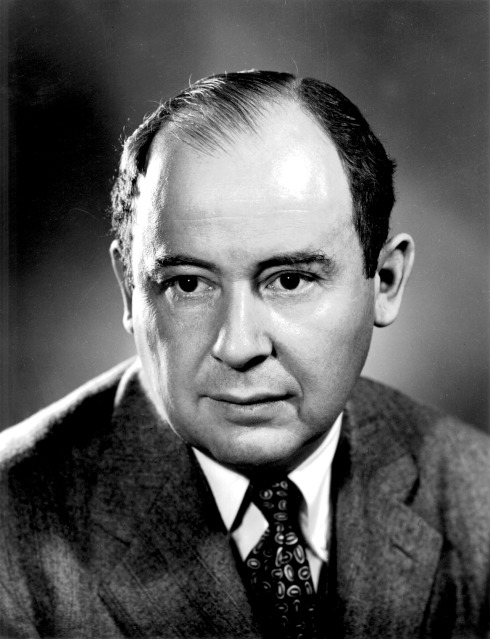
\includegraphics[height=4cm]{figs/von-neumann.jpg}
    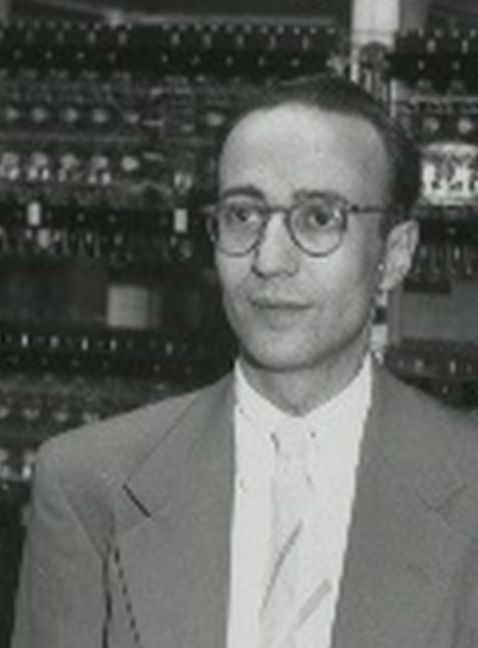
\includegraphics[height=4cm]{figs/goldstine.jpg}

    {\small ``Numerical Inverting of Matrices of High Order'' (1947)}
  \end{center}

  \begin{quote}
    ... matrices of the orders 15, 50, 150 can usually be inverted
    with a (relative) precision of 8, 10, 12 decimal digits less,
    respectively, than the number of digits carried throughout.
  \end{quote}

\end{frame}


\begin{frame}
  \frametitle{Some history: Turing}
  
  \begin{center}
    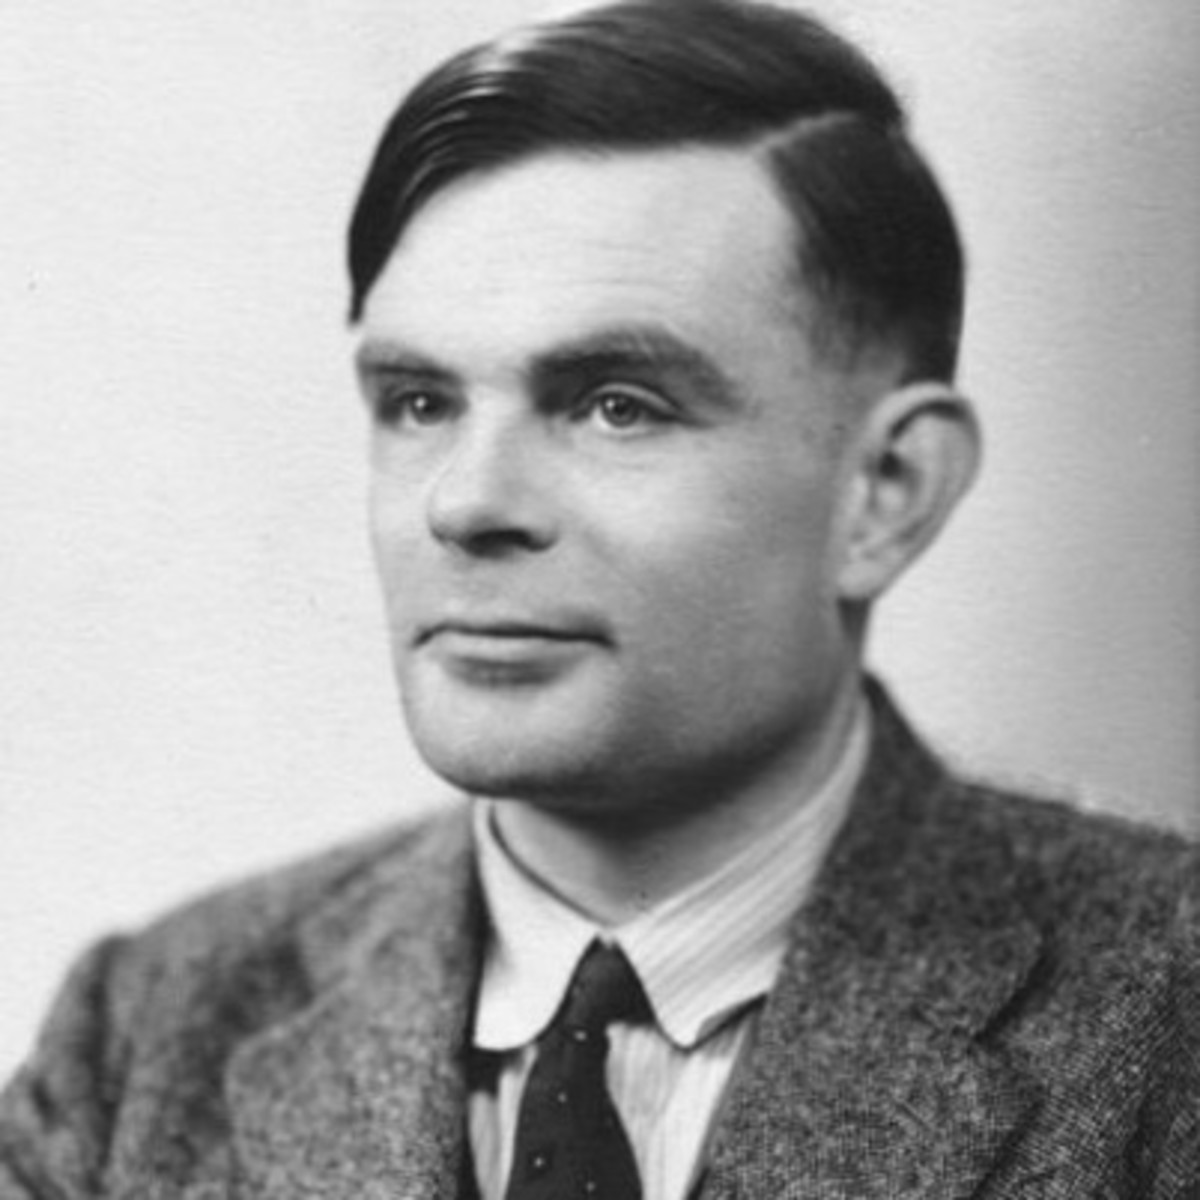
\includegraphics[height=5cm]{figs/turing.jpg}

    {\small ``Rounding-Off Errors in Matrix Processes'' (1948)}
  \end{center}

  Carrying $d$ digits is equivalent to changing input
  data in the $d$th place (backward error analysis).
\end{frame}


\begin{frame}
  \frametitle{Some history: Wilkinson}
  
  \begin{center}
    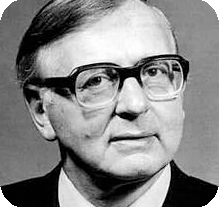
\includegraphics[height=3cm]{figs/wilkinson.jpg}

    {\small ``Error Analysis of Direct Methods of Matrix
    Inversion'' (1961) \\ Modern error analysis of Gaussian elimination}
  \end{center}

  \begin{quote}
    For his research in numerical analysis to facilitiate the use of
    the high-speed digital computer, having received special
    recognition for his work in computations in linear algebra and
    ``backward'' error analysis. \hfill --- 1970 Turing Award citation
  \end{quote}
\end{frame}

\begin{frame}
  \frametitle{Some history: Kahan}
  
  \begin{center}
    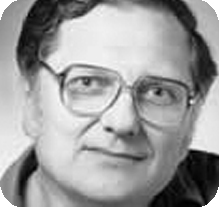
\includegraphics[height=3cm]{figs/kahan.jpg}

    IEEE-754/854 (1985, revised 2008)
  \end{center}

  \begin{quote}
    For his fundamental contributions to numerical analysis. One of
    the foremost experts on floating-point computations. Kahan has
    dedicated himself to ``making the world safe for numerical
    computations.''
    \hfill --- 1989 Turing Award citation
  \end{quote}
\end{frame}


\begin{frame}
  \frametitle{IEEE floating point reminder}

  Normalized numbers:
  \[
    (-1)^s \times (1.b_1 b_2 \ldots b_p)_2 \times 2^e
  \]
  Have 32-bit single, 64-bit double numbers consisting of
  \begin{itemize}
  \item Sign $s$
  \item Precision $p$ ($p = 23$ or $52$)
  \item Exponent $e$ ($-126 \leq e \leq 126$ or $-1022 \leq e \leq 1023$)
  \end{itemize}

  \vspace{5mm}
  Questions:
  \begin{itemize}
  \item What if we can't represent an exact result?
  \item What about $2^{e_{\max}+1} \leq x < \infty$ or $0 \leq x < 2^{e_{\min}}$?
  \item What if we compute $1/0$?
  \item What if we compute $\sqrt{-1}$?
  \end{itemize}
\end{frame}


\begin{frame}
  \frametitle{Rounding}

  Basic ops ($+, -, \times, /, \sqrt{}$), require {\em correct rounding}
  \begin{itemize}
  \item As if computed to infinite precision, then rounded.
    \begin{itemize}
    \item Don't actually need infinite precision for this!
    \end{itemize}
  \item Different rounding rules possible:
    \begin{itemize}
    \item Round to nearest even (default)
    \item Round up, down, toward 0 -- error bounds and intervals
    \end{itemize}
  \item If rounded result $\neq$ exact result, have {\em inexact exception}
    \begin{itemize}
    \item Which most people seem not to know about...
    \item ... and which most of us who do usually ignore
    \end{itemize}
  \item 754-2008 {\em recommends} (does not require) correct rounding
    for a few transcendentals as well (sine, cosine, etc).
  \end{itemize}

\end{frame}


\begin{frame}
  \frametitle{Denormalization and underflow}

  Denormalized numbers:
  \[
    (-1)^s \times (0.b_1 b_2 \ldots b_p)_2 \times 2^{e_{\min}}
  \]
  \begin{itemize}
  \item Evenly fill in space between $\pm 2^{e_{\min}}$
  \item Gradually lose bits of precision as we approach zero
%  \item Required to guarantee $x-y = 0 \implies x = y$
  \item Denormalization results in an {\em underflow exception}
    \begin{itemize}
    \item Except when an exact zero is generated
    \end{itemize}
  \end{itemize}
  
\end{frame}


\begin{frame}
  \frametitle{Infinity and NaN}

  Other things can happen:
  \begin{itemize}
  \item $2^{e_{\max}} + 2^{e_{\max}}$ generates $\infty$ ({\em overflow exception})
  \item $1/0$ generates $\infty$ ({\em divide by zero exception})
    \begin{itemize}
    \item ... should really be called ``exact infinity'' exception
    \end{itemize}
  \item $\sqrt{-1}$ generates Not-a-Number ({\em invalid exception})
  \end{itemize}
  But every basic operation produces {\em something} well defined.
\end{frame}


\begin{frame}
  \frametitle{Basic rounding model}

  Model of roundoff in a basic op:
  \[
    \fl(a \odot b) = (a \odot b)(1 + \delta), \quad
    |\delta| \leq \macheps.
  \]
  \begin{itemize}
  \item This model is {\em not} complete
    \begin{itemize}
    \item Optimistic: misses overflow, underflow, divide by zero
    \item Also too pessimistic -- some things are done exactly!
    \item Example: $2x$ exact, as is $x+y$ if $x/2 \leq y \leq 2x$
    \end{itemize}
  \item But useful as a basis for backward error analysis
  \end{itemize}
\end{frame}


\begin{frame}[fragile]
  \frametitle{Example: Horner's rule}

Evaluate $p(x) = \sum_{k=0}^n c_k x^k$:
\begin{lstlisting}
p = c(n)
for k = n-1 downto 0
  p = x*p + c(k)
\end{lstlisting}

\vspace{5mm}
Can show backward error result:
\[
  \fl(p) = \sum_{k=0}^n \hat{c}_k x^k
\]
where $|\hat{c}_k-c_k| \leq (n+1) \macheps |c_k|$.

\vspace{5mm}
Backward error + sensitivity gives forward error.  Can even
compute running error estimates!

\end{frame}


\begin{frame}[fragile]
  \frametitle{Hooray for the modern era!}

  \begin{itemize}
  \item Almost everyone implements IEEE 754 (at least 1985)
    \begin{itemize}
    \item Old Cray arithmetic is essentially extinct
    \end{itemize}
  \item We teach backward error analysis in basic classes
  \item Good libraries for linear algebra, 
        elementary functions
  \end{itemize}
\end{frame}


\begin{frame}[fragile]
  \frametitle{Back to the future?}

  \begin{itemize}
  \item Almost everyone implements IEEE 754 (at least 1985)
    \begin{itemize}
    \item Old Cray arithmetic is essentially extinct
    \item But GPUs may lack gradual underflow
    \item And it's impossible to write portable exception handlers
    \item And even with C99, exception flags may be inaccessible
    \item And some features might be slow 
    \item And the compiler might not do what you expected
    \end{itemize}
  \item We teach backward error analysis in basic classes
    \begin{itemize}
    \item ... which are often no longer required!
    \item And anyhow, backward error analysis isn't everything.
    \end{itemize}
  \item Good libraries for linear algebra, 
        elementary functions
    \begin{itemize}
    \item But people will still roll their own.
    \end{itemize}
  \end{itemize}

\end{frame}


\begin{frame}
  \frametitle{Arithmetic speed}

  Single precision is faster than double precision
  \begin{itemize}
  \item Actual arithmetic cost may be comparable (on CPU)
  \item But GPUs generally prefer single
  \item And SSE instructions do more per cycle with single
  \item And memory bandwidth is lower
  \end{itemize}
  NB: There is a half-precision type (use for storage only!)
  
\end{frame}


\begin{frame}
  \frametitle{Mixed-precision arithmetic}

  Idea: use double precision only where needed
  \begin{itemize}
  \item Example: iterative refinement and relatives
  \item Or use double-precision arithmetic between
    single-precision representations (may be a good idea regardless)
  \end{itemize}
\end{frame}


\begin{frame}
  \frametitle{Example: Mixed-precision iterative refinement}

\begin{tabbing}
\qquad \= \hspace{4cm} \= \kill
Factor $A = LU$ \>\> $O(n^3)$ single-precision work\\
Solve $x = U^{-1} (L^{-1} b)$ \>\> $O(n^2)$ single-precision work \\
$r = b-Ax$ \>\> $O(n^2)$ double-precision work \\
While $\|r\|$ too large \\
\> $d = U^{-1} (L^{-1} r)$ \> $O(n^2)$ single-precision work\\
\> $x = x+d$ \> $O(n)$ single-precision work \\
\> $r = b-Ax$ \> $O(n^2)$ double-precision work
\end{tabbing}

\end{frame}


\begin{frame}[fragile]
  \frametitle{Example: Helpful extra precision}

\begin{lstlisting}
/*
 * Assuming all coordinates are in [1,2), check on which
 * side of the line through A and B is the point C.
 */
int check_side(float ax, float ay, float bx, float by, 
               float cx, float cy)
{
    double abx = bx-ax, aby = by-ay;
    double acx = cx-ax, acy = cy-ay;
    double det = acx*aby-abx*aby;
    if (det == 0) return  0;
    if (det <  0) return -1;
    if (det >  0) return  1;
}
\end{lstlisting}
This is not robust if the inputs are double precision!
\end{frame}


\begin{frame}
  \frametitle{Single or double?}

  What to use for:
  \begin{itemize}
  \item Large data sets?  (single for performance, if possible)
  \item Local calculations?  (double by default, except GPU?)
  \item Physically measured inputs?  (probably single)
  \item Nodal coordinates?  (probably single)
  \item Stiffness matrices?  (maybe single, maybe double)
  \item Residual computations?  (probably double)
  \item Checking geometric predicates?  (double or more)
  \end{itemize}
\end{frame}


\begin{frame}[fragile]
  \frametitle{Simulating extra precision}
  
  What if we want higher precision than is fast?
  \begin{itemize}
  \item Double precision on a GPU?
  \item Quad precision on a CPU?
  \end{itemize}
  Can simulate extra precision.  Example:
\begin{lstlisting}
  if abs(a) < abs(b) { swap(&a, &b); }
  double s1 = a+b;         /* May suffer roundoff */
  double s2 = (a-s1) + b;  /* No roundoff! */
\end{lstlisting}
  Idea applies more broadly (Bailey, Bohlender, Dekker, Demmel, Hida,
  Kahan, Li, Linnainmaa, Priest, Shewchuk, ...)
  \begin{itemize}
  \item Used in fast extra-precision packages
  \item And in robust geometric predicate code
  \item And in XBLAS
  \end{itemize}

\end{frame}


\begin{frame}[fragile]
  \frametitle{Exceptional arithmetic speed}

  Time to sum 1000 doubles on my laptop:
  \begin{itemize}
  \item Initialized to 1: 1.3 microseconds
  \item Initialized to inf/nan: 1.3 microseconds
  \item Initialized to $10^{-312}$: 67 microseconds
  \end{itemize}
  $50 \times$ performance penalty for gradual underflow!

  \vspace{5mm}
  Why worry?  Some GPUs don't support gradual underflow
  at all! \\
One reason:
\begin{lstlisting}
if (x != y)
    z = x/(x-y);
\end{lstlisting}

Also limits range of simulated extra precision.

\end{frame}


\begin{frame}
  \frametitle{Exceptional algorithms, take 2}

  A general idea (works outside numerics, too):
  \begin{itemize}
  \item Try something fast but risky
  \item If something breaks, retry more carefully
  \end{itemize}
  If risky usually works and doesn't cost too much extra,
  this improves performance.

  \vspace{1cm}
  (See Demmel and Li, and also Hull, Farfrieve, and Tang.)

\end{frame}


\begin{frame}
  \frametitle{Parallel problems}
  
  What goes wrong with floating point in parallel (or just high performance)
  environments?
\end{frame}


\begin{frame}
  \frametitle{Problem 0: Mis-attributed Blame}

  \begin{quote}
    To blame is human.  To fix is to engineer. \\ \hfill --- Unknown
  \end{quote}
  
  Three variants:
  \begin{itemize}
  \item ``I probably don't have to worry about floating point error.''
  \item ``This is probably due to floating point error.''
  \item ``Floating point error makes this untrustworthy.''
  \end{itemize}
\end{frame}


\begin{frame}
  \frametitle{Problem 1: Repeatability}

  Floating point addition is {\em not} associative:
  \[
    \fl(a + \fl(b + c)) \neq \fl(\fl(a + \b) + c)
  \]

  So answers depends on the inputs, but also
  \begin{itemize}
  \item How blocking is done in multiply or other kernels
  \item Maybe compiler optimizations
  \item Order in which reductions are computed
  \item Order in which critical sections are reached
  \end{itemize}

  \vspace{4mm}
  Worst case: with nontrivial probability we get an answer
  too bad to be useful, not bad enough for the program to barf ---
  and garbage comes out.

\end{frame}


\begin{frame}
  \frametitle{Problem 1: Repeatability}

  What can we do?
  \begin{itemize}
  \item Apply error analysis agnostic to ordering
  \item Write a slower version with specific ordering for debugging
  \item Soon: Call the {\em reproducible BLAS}
  \end{itemize}
  Note: new {\tt two\_sum} operation under discussion in IEEE 754
  committee should make fast reproducibility (and double-double) easier.
\end{frame}


\begin{frame}
  \frametitle{Problem 2: Heterogeneity}

  \begin{itemize}
  \item Local arithmetic faster than communication
  \item So be redundant about some computation
  \item What if the redundant computations are on different HW?
    \begin{itemize}
    \item Different nodes in the cloud?
    \item GPU and CPU?
    \end{itemize}
  \item Problem: different exception handling on different nodes
  \item Problem: different branches due to different rounding
  \end{itemize}
\end{frame}


\begin{frame}
  \frametitle{Problem 2: Heterogeneity}

  What can we do?
  \begin{itemize}
  \item Avoid FP-dependent branches
  \item Communicate FP results affecting branches
  \item Use reproducible kernels
  \end{itemize}
  
\end{frame}


\begin{frame}
  \frametitle{Recap}

  So why care about the vagaries of floating point?
  \begin{itemize}
  \item Might actually care about error analysis
  \item Or using single precision for speed
  \item Or maybe just reproducibility
  \item Or avoiding crashes from inconsistent decisions!
  \end{itemize}

  \vspace{5mm}
  Start with ``What Every Computer Scientist Should Know About Floating Point
  Arithmetic'' (David Goldberg, with an addendum by Doug Priest).  It's in
  the back of Patterson-Hennessey.

\end{frame}

\end{document}
